\section{Simulator Validation}	\label{sec:valid}
%
To validate the correctness and accuracy of EBeSS, we compare the execution parameters of EBeSS with a real NVP-based system prototype~\cite{wang2017a130nm} as shown in Figure~\ref{fig:HardwarePrototype}.
A bridge monitoring application and several independent tasks are executed to compare the performance and energy parameters.

% hardware parameters
\subsection{System configurations}
The configuration of the system prototype is listed in Table~\ref{}. 
This prototype is an solar-powered system, which contains a nonvolatile processor (NVP)~\cite{wang20123us,Liu2015Ambient}, a nonvolatile radio transmitter (NVRF)~\cite{wang2017a130nm} and several volatile sensors.

\begin{figure}[!htpb]
	\centering
	\vspace{-5pt}
	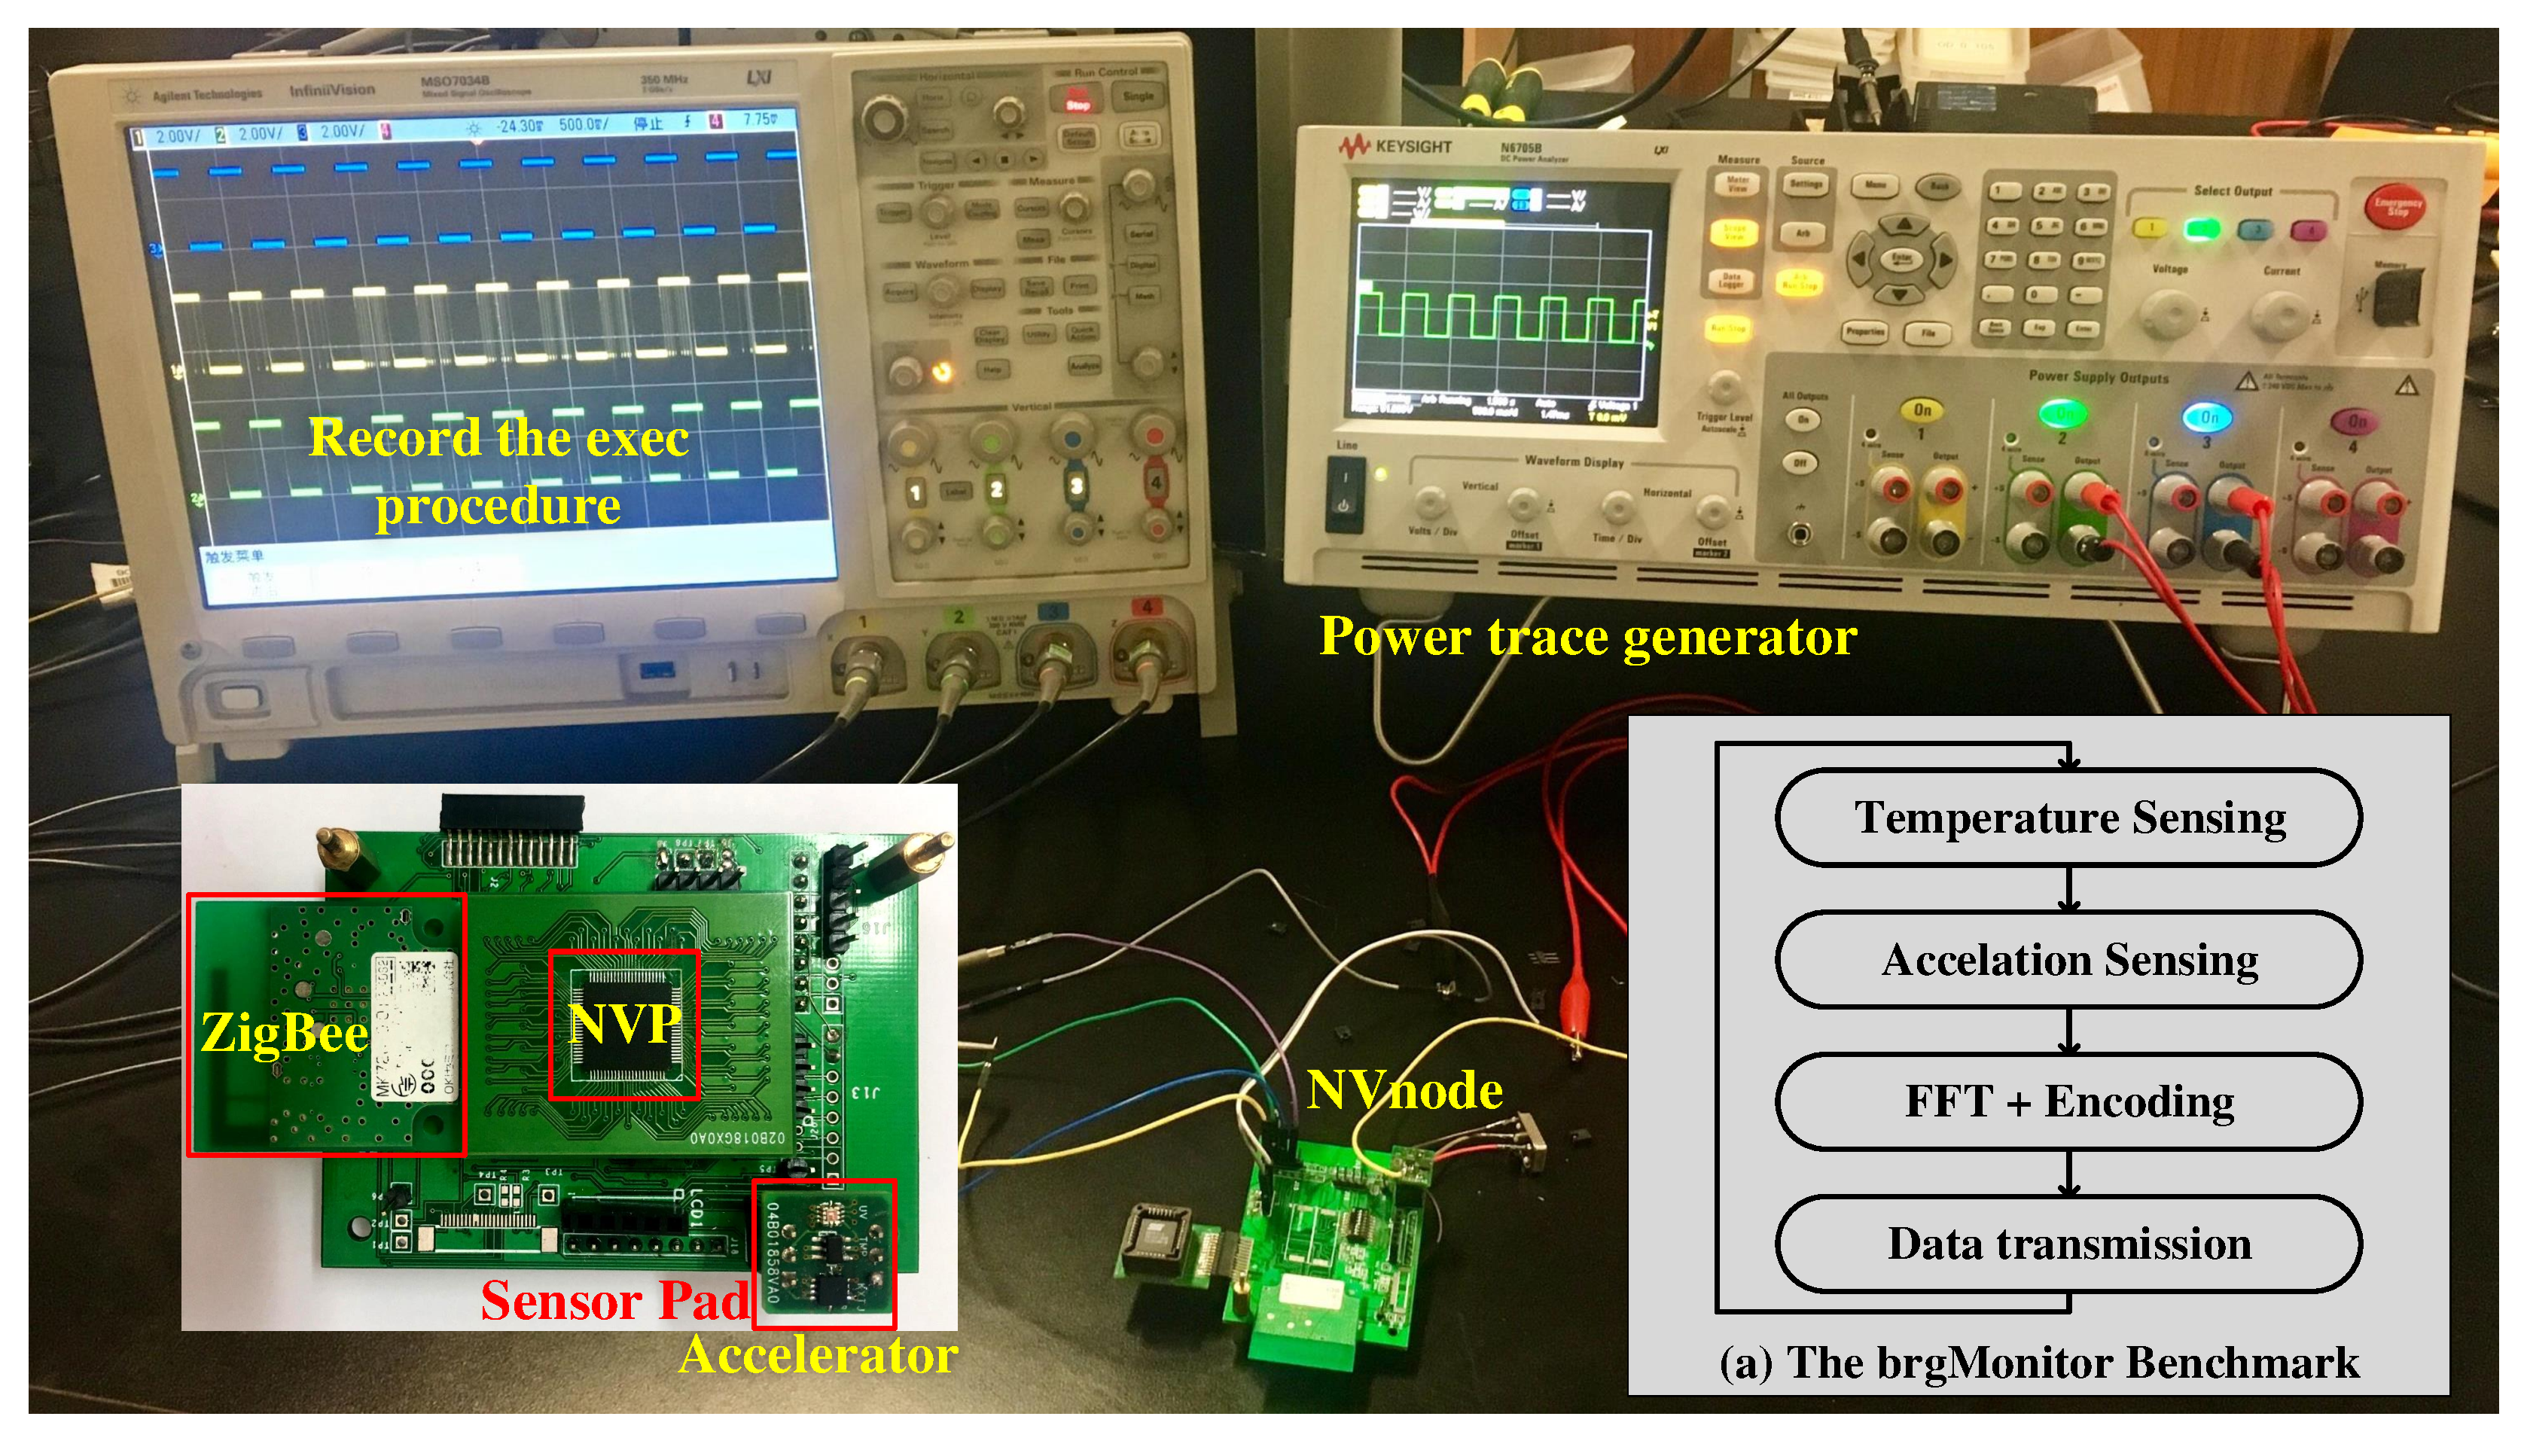
\includegraphics[width=0.48\textwidth]{HardwarePrototype}
	\vspace{-5pt}
	\caption{The hardware prototype used to validate EBeSS simulator. A real bridge monitoring benchmark is utilized to validate the simulator.}	\label{fig:HardwarePrototype}
\end{figure}

NVP enables a two-threshold backup/restore energy managing strategy (\emph{2-thr})~\cite{wang20123us,gu2016nvpsim}, where a lower threshold $V_{low}$ and a higher threshold $V_{high}$ are defined.
When the supply voltage falls below $V_{low}$, the processor immediately backup the execution status to NVM with the help of a control circuit.
When the supply voltage raises above $V_{high}$, the processor restarts and restores all the states and keep on progress.

NVRF is a nonvolatile interface that can automatically recover the radio transmitter and retransmit the uncompleted packet transmission after outages.
Inheriting the two voltage thresholds in \emph{2-thr}, NVRF can backup the configurations of the radio transmitter when the voltage is lower than $V_{low}$, and will reinitialize the transmitter states, resume the configurations and restart the uncompleted transmission.

In addition, the prototype also contains a thermometer and an accelerometer. 
The capacitor is $15uF$. 
All the above hardware parameters are listed in Table~\ref{}.
The power profiles are solar power traces from MIDC database of NREL Solar Radiation Research Laboratory~\cite{midc2015solar}.

% hardware parameters
\subsection{Application Validation}
We compare the simulation result with the hardware execution result using a real IoT application, bridge monitoring application (\emph{brgMonitor}).
The work flow of \emph{brgMonitor} is shown in Figure~\ref{fig:HardwarePrototype}.
The device executes a 'sense-process-transmit' cycle to collect bridge health related parameters.
The execution time and energy consumption comparison is shown in Table~\ref{}.
% The error is ...

Furthermore, we also evaluate the correctness of EBeSS with multiple small tasks in Table~\ref{}.
The maximum error is limited within XXX.

%\begin{table}[t]
	\begin{center}
		%\vspace{-0pt}
		\caption{Parameter Settings of NVP System Prototype~\cite{Liu2015Ambient}.} \label{tab:valid-param}
		%\vspace{-5pt}
		\Fsize{8}
		\renewcommand{\arraystretch}{1.5}
		%\setlength{\tabcolsep}{1pt}
		\begin{tabular}{Ic|c|c|c|c|cI}
			\Xhline{1.2pt}
			Param.	& Oper. Freq.	& power	& Mem	& RegFile	& Cap.\\
			\Xhline{1pt}
			Value	& $1$MHz	& $0.16$mW	& $512$KB	& $128$B	& $10\mu F$\\
			\Xhline{1.2pt}
		\end{tabular}
		\vspace{-15pt}
	\end{center}
\end{table} 
%\begin{table}[t]
	\begin{center}
	\caption{Comparison Between EBeSS and NVP Prototype.} \label{tab:valid-result}
	\vspace{-10pt}
	\Fsize{8}
	\renewcommand{\arraystretch}{1.5}
	\setlength{\tabcolsep}{1.8pt}
	\begin{tabular}{Ic|cIc|c|cIc|c|cIc|c|cI}
		\Xhline{1.2pt}
		\multicolumn{2}{IcI}{}	& \multicolumn{3}{cI}{FFT}		& \multicolumn{3}{cI}{QUEENS}	& \multicolumn{3}{cI}{SORT} \\
		\Xhline{1.2pt}

		Power	& Metrics		& Sim.	& Mea.	& Err.			& Sim.	& Mea.	& Err.			& Sim.	& Mea.	& Err. \\

		\Xhline{1pt}
		\multirow{2}[1.2]{*}{Trace 1}
			& engy./uJ		& 4.21	& 4.02	& 4.51\%		& 7.61	& 7.45	& 2.10\%		& 29.2	& 26.9	& 7.88\% \\
		\cline{2-11}
			& time/ms		& 39.2	& 36.7	& 6.38\%		& 77.4	& 74.3	& 4.01\%		& 266	& 253	& 4.89\% \\

		\Xhline{1pt}
		\multirow{2}[1.2]{*}{Trace 2}
			& engy./uJ		& 2.98	& 2.93	& 1.68\%		& 5.14	& 4.97	& 3.31\%		& 16.2	& 15.4	& 4.94\% \\
		\cline{2-11}
			& time/ms		& 21.2	& 20.6	& 2.83\%		& 51.1	& 49.6	& 2.94\%		& 172	& 166	& 3.49\% \\

		\Xhline{1pt}
		\multirow{2}[1.2]{*}{Trace 3}
			& engy./uJ		& 2.19	& 2.15	& 1.83\%		& 2.97	& 2.91	& 2.02\%		& 10.9	& 10.6	& 2.75\% \\
		\cline{2-11}
			& time/ms		& 14.5	& 14.4	& 0.69\%		& 24.5	& 24.5	& 0.00\%		& 91.1	& 90.2	& 0.99\% \\

		\Xhline{1.2pt}
	\end{tabular}
	\end{center}
	\vspace{-20pt}
\end{table} 

\begin{comment}
\bibliographystyle{ACM-Reference-Format}
\bibliography{references} 
\end{comment}